% Target: NeurIPS 2027 Datasets & Benchmarks track.
% To build with the official template, replace the next two lines with the track's style, e.g.
%   \documentclass{article}\usepackage[preprint]{neurips_2027}   (and the D&B option the call specifies)
\documentclass[11pt]{article}
\usepackage[margin=1in]{geometry}
\usepackage[utf8]{inputenc}
\usepackage[T1]{fontenc}
\makeatletter\@namedef{ver@epstopdf-base.sty}{2020/01/01}\makeatother % local TinyTeX lacks grfext; harmless for PDF-only builds
\usepackage{booktabs,graphicx,amsmath,amssymb,xcolor,url}
\usepackage[numbers]{natbib}
\newcommand{\pending}[1]{\textcolor{orange}{[PENDING: #1]}}
\newcommand{\tautwo}{$\tau^2$-bench}

\title{Did It Go Through? A Benchmark of Uncertain-Outcome Faults\\for Tool-Using Agents}
\author{Anonymous Authors}
\date{}

\begin{document}
\maketitle
\sloppy

\begin{abstract}
When a state-changing tool call fails with an uncertain outcome (for example, a timeout after the request was sent), retrying blindly can duplicate a booking, an order or a payment, while giving up can silently drop it. The only policy that is correct in both cases is to \emph{check the state, then decide}. We introduce \textbf{Uncertain-Outcome Faults (UOF)}, a benchmark built on BFCL v4 multi-turn tasks and \tautwo{} airline. Each fault comes as a pair of \emph{outcome twins} with an identical observable history, in which the faulted call either was or was not applied. A blind policy therefore scores at most 0.5, and grading is by execution against the ground-truth end state. Across Qwen3 models from 4B to 30B parameters, with or without an explicit instruction, and after state-of-the-art corrective training on standard faults, agents re-issue the uncertain call in 71--100\% of cases and score at the blind-retry level (0.47--0.53). In six pre-registered training studies we then locate what does and does not transfer to unseen APIs. Checking transfers when the error text states the uncertainty. Reading the check transfers only with diverse training APIs. Recognising the risk behind a plain ``request timed out'' stays tied to the APIs seen in training, even when MCP-style idempotency annotations are shown. Training on procedurally generated stateful APIs is the first intervention that transfers this recognition to an unseen real API class (+0.10 over three seeds), and doubling API diversity at fixed data size adds +0.06. The rule it learns follows verb meaning rather than side effects and fails zero-shot on \tautwo{} cancellations; a verb-agnostic check-all-writes rule with persistent-failure continuations fixes this, transferring zero-shot to \tautwo{} ($+0.82$ checking, 86\% of cancellations) and to held-out BFCL ($+0.08$) without regressing the original fault suites (2 seeds). We release the benchmark, graders, data builders, all protocols and per-episode traces.
\end{abstract}

\section{Introduction}
Tool-using language-model agents increasingly act on real systems: they book, order, pay, message and cancel. Real systems fail ambiguously. A request can time out \emph{after} the server applied it, so the client cannot tell whether the action happened. Distributed-systems practice has a standard answer: idempotency keys and read-after-write verification \citep{TODO_idempotency}. By contrast, agent benchmarks and corrective-training methods mostly consider faults with an unambiguous correct response: retry a transient outage, switch to a backup endpoint, repair a wrong argument, or escalate \citep{TODO_bfcl,TODO_taubench,TODO_cso}.

Our starting point was a negative result. On BFCL multi-turn tasks with standard injected faults, a strong corrective-training pipeline (corrective SFT followed by CSO-style, rollout-verified step DPO, replicated over three seeds) leaves only about $+0.03$ of recoverable held-out headroom. Most remaining failures fail even without faults. Standard fault suites are close to saturated for this purpose. We therefore turned to the fault class where retrying is \emph{harmful}: the uncertain commit.

\paragraph{Contributions.}
\begin{enumerate}
\item \textbf{The UOF benchmark} (\S\ref{sec:bench}).
  \begin{itemize}
  \item Outcome-twin faults on 116 BFCL tasks, including a 73-task \emph{decisive} subset whose outcome can be read from a single check, plus 13 \tautwo{} airline write events and 36 repeat-safe controls.
  \item Error wordings that shift at test time, including a realistic \emph{implicit} timeout.
  \item Controls where retrying is correct, so that over-checking is measured.
  \item Every instance is constructed and validated by execution; scripted reference policies separate exactly.
  \end{itemize}
\item \textbf{A capability gap} (\S\ref{sec:gap}). Neither prompting nor scale up to 30B parameters closes it, and neither does strong corrective training on standard faults.
\item \textbf{A transfer analysis of training} (\S\ref{sec:transfer}). Six pre-registered studies with matched baselines separate three skills (checking, reading the check, and recognising implicit risk) and show which training signals move each.
\item \textbf{Open artefacts}: code, graders, training-data builders, all pre-registrations with their edit logs, and checksummed per-episode traces.
\end{enumerate}

\section{The UOF benchmark}\label{sec:bench}
\paragraph{Environments.}
\begin{itemize}
\item \textbf{BFCL v4 multi-turn base} \citep{TODO_bfcl} (bfcl-eval 2026.3.23): executable Python API backends for 8 API classes. Each episode is one user turn, with earlier turns shown as executed history. Grading requires every public attribute of every involved API instance to equal the ground-truth end state.
\item \textbf{\tautwo{} airline} \citep{TODO_tau2} (commit \texttt{c06b07dd}): a second, independent codebase, graded by database hash. It is used only for zero-shot evaluation.
\end{itemize}

\paragraph{Outcome twins.} The first call to the task's \emph{fault target} $f$ (its first state-changing call) returns an error.
\begin{itemize}
\item In \textbf{ACa}, $f$ was executed; in \textbf{ACl}, it was not.
\item The observation is identical in both, so any policy that ignores the state succeeds in at most one twin.
\item Correct behaviour is to check the state, then continue (ACa) or re-issue $f$ (ACl).
\end{itemize}

\paragraph{Instance selection by execution.} A BFCL task is
\begin{itemize}
\item \emph{diagnostic} if executing $f$ twice breaks the end state and some read-only function shows the difference (116 of 398 usable tasks);
\item \emph{decisive} if some argument value of $f$ appears in one read-only output only when $f$ was applied, so the outcome is readable from one check without remembering the earlier state (73 tasks).
\end{itemize}
The same procedure on \tautwo{} airline yields 13 non-idempotent, readable write events (11 \texttt{cancel\_reservation}, which refunds again on every call; 2 \texttt{book\_reservation}) and 36 repeat-safe controls.

\paragraph{Wordings.} \emph{explicit}: ``\ldots the operation may or may not have been applied''; \emph{para} (never used for training): ``\ldots the request might already have been processed''; \emph{implicit} (never used for training): ``Error: the request timed out.''

\paragraph{Validation.} Scripted policies separate exactly on every instance and wording (Table~\ref{tab:valid}).

\begin{table}[t]\centering\small
\caption{Scripted validation: successes / instances.}\label{tab:valid}
\begin{tabular}{lcccc}\toprule
policy & BFCL ACa & BFCL ACl & \tautwo{} ACa & \tautwo{} ACl\\\midrule
verify-then-decide & 116/116 & 116/116 & 39/39 & 39/39\\
blind retry & 0/116 & 116/116 & 0/39 & 39/39\\
never retry & 116/116 & 0/116 & 39/39 & 0/39\\
escalate & 0/116 & 0/116 & -- & --\\\bottomrule
\end{tabular}\end{table}

\paragraph{Metric and controls.}
\begin{itemize}
\item \textbf{Primary metric:} mean success over ACa and ACl, restricted to tasks the policy (or, for transfer comparisons, a fixed reference policy) solves fault-free. Blind retry scores 0.5; verify-then-decide scores 1.0.
\item \textbf{Controls:} S0 (fault-free), S1 (transient outage, where retrying is correct) and the original BFCL fault suites. Together these show whether a method checks needlessly or regresses.
\end{itemize}

\section{The gap: prompting and scale do not help}\label{sec:gap}
Table~\ref{tab:leader} and Figure~\ref{fig:gap} summarise the untrained policies.
\begin{itemize}
\item Every untrained policy scores at the blind-retry level on every wording: Qwen3 4B, 8B and 30B-A3B; the corrective-SFT policy $\pi_0$; and the CSO-style verified-DPO baseline B.
\item An explicit instruction to check after uncertain failures helps only the 30B model, and only partially (0.65 on the paraphrase). Even when that model checks, it often re-issues the call after reading a state that already shows it.
\end{itemize}

\begin{figure}[t]\centering
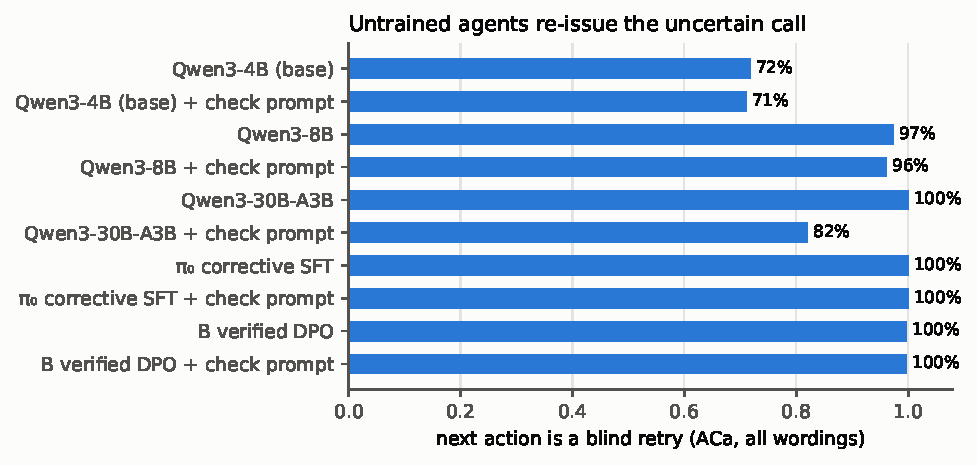
\includegraphics[width=0.62\linewidth]{figures/fig1_blind_retry.pdf}
\caption{Share of applied-twin episodes whose next action is a blind retry (all wordings).}\label{fig:gap}
\end{figure}

\begin{table}[t]\centering\scriptsize
\caption{UOF leaderboard (BFCL, 116 diagnostic tasks; AC success given S0). Trained rows: mean of 3 seeds. \tautwo{}: check rate after the implicit error on 13 diagnostic airline writes.}\label{tab:leader}
\resizebox{\linewidth}{!}{\begin{tabular}{lccccccc}\toprule
policy & seeds & S0 & S1$|$S0 & explicit & para & implicit & \tautwo{} check\\ \midrule
Qwen3-4B-Instruct-2507 (base) & 1 & 0.810 & 0.968 & 0.489 & 0.495 & 0.495 & --\\
Qwen3-4B-Instruct-2507 (base) + check prompt & 1 & 0.828 & 0.979 & 0.500 & 0.505 & 0.495 & --\\
Qwen3-8B (no thinking) & 1 & 0.759 & 0.943 & 0.472 & 0.489 & 0.477 & --\\
Qwen3-8B (no thinking) + check prompt & 1 & 0.759 & 0.943 & 0.489 & 0.494 & 0.494 & --\\
Qwen3-30B-A3B-Instruct-2507 (FP8) & 1 & 0.888 & 1.000 & 0.500 & 0.500 & 0.500 & --\\
Qwen3-30B-A3B-Instruct-2507 (FP8) + check prompt & 1 & 0.897 & 1.000 & 0.534 & 0.649 & 0.500 & --\\
$\pi_0$ (corrective SFT) & 1 & 0.845 & 1.000 & 0.500 & 0.500 & 0.500 & --\\
$\pi_0$ (corrective SFT) + check prompt & 1 & 0.845 & 1.000 & 0.500 & 0.500 & 0.500 & --\\
B: CSO-style verified DPO & 1 & 0.888 & 1.000 & 0.510 & 0.510 & 0.510 & --\\
B: CSO-style verified DPO + check prompt & 1 & 0.888 & 0.981 & 0.505 & 0.505 & 0.505 & --\\
\midrule
SYN-old (synthetic APIs, retry convention) & 3 & 0.862 & 0.987 & 0.656 & 0.674 & 0.631 & 0.000\\
\midrule
SYN-32 (32 synthetic classes, IAR) & 3 & 0.859 & 0.997 & 0.694 & 0.778 & 0.676 & 0.000\\
SYN-64 (64 synthetic classes, IAR) & 3 & 0.856 & 1.000 & 0.729 & 0.805 & 0.696 & 0.026\\
\midrule
scripted verify-then-decide (reference) & - & 1.000 & 1.000 & 1.000 & 1.000 & 1.000 & 1.000\\
scripted blind retry (reference) & - & 1.000 & 1.000 & 0.500 & 0.500 & 0.500 & 0.000\\
\bottomrule\end{tabular}
}
\end{table}

\section{What training transfers}\label{sec:transfer}
\paragraph{Protocol.}
\begin{itemize}
\item All studies start from $\pi_B$ ($\pi_0$ plus B, merged) and use LoRA SFT or DPO.
\item Each study compares against a \emph{matched} baseline that differs only in the property under test.
\item The primary metric, gate and claim rule of each study were fixed before training (\S\ref{sec:method}).
\item Evaluation uses API classes held out from training, and wordings never trained on.
\end{itemize}

\paragraph{Checking transfers; reading needs diversity.}
\begin{itemize}
\item \emph{Outcome-twin training} (check at the error, then decide from the check) on 2 API classes raises checking on unseen classes from 0\% to 58\%. Post-check decisions there, however, are at chance (28/67).
\item With 4 training classes and plain SFT, a model checks in 76/76 held-out-class episodes on the unseen paraphrase, and decides correctly in 64/76.
\item Adding one-sentence \emph{evidence rationales} to the targets hurts: $-0.091$ [$-0.148$, $-0.034$], with over-checking on fault-free episodes.
\end{itemize}

\paragraph{Implicit risk is tied to API identity.}
\begin{itemize}
\item Training the rule ``a timeout on a state-changing call means check'' makes models check after the plain implicit timeout on 96\% of new tasks \emph{within} the trained API classes, but on 0/76 episodes of a held-out class.
\item Printing execution-derived MCP-style annotations (\texttt{readOnlyHint}, \texttt{idempotentHint}) \citep{TODO_mcp} in every tool description changes this to only 2/76.
\end{itemize}

\paragraph{Synthetic API diversity transfers the rule, and scales.}
\begin{itemize}
\item We generate stateful APIs that vary domain, verbs, naming and output format while fixing semantics (create is non-idempotent; set and remove are idempotent), and verify every training decision by execution.
\item \textbf{32 classes, 3 seeds:} held-out-class implicit success $0.610$ vs $0.510$ for an identical-data control trained under the old ``retry'' convention, $+0.099$ [0.024, 0.171], positive in 3/3 seeds. The unseen paraphrase gains $+0.171$, with no regression on the original suites.
\item \textbf{64 classes at the same data size:} a further $+0.058$ [0.014, 0.110] (Figure~\ref{fig:scale}).
\item One training seed fails in both configurations (8/76 checks), so reliability remains open.
\end{itemize}

\begin{figure}[t]\centering
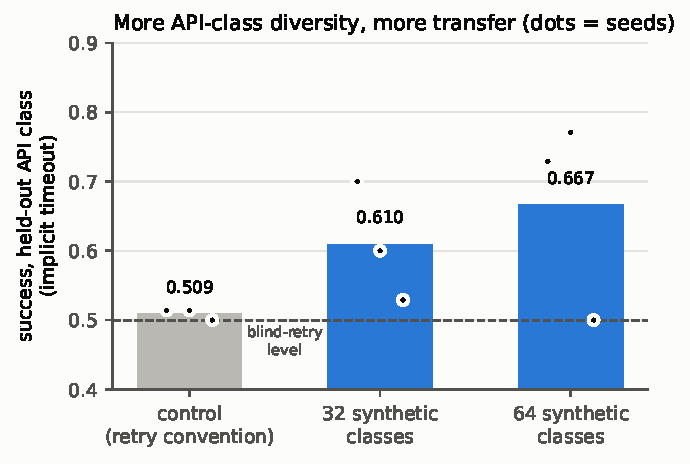
\includegraphics[width=0.48\linewidth]{figures/fig2_transfer_scaling.pdf}\hfill
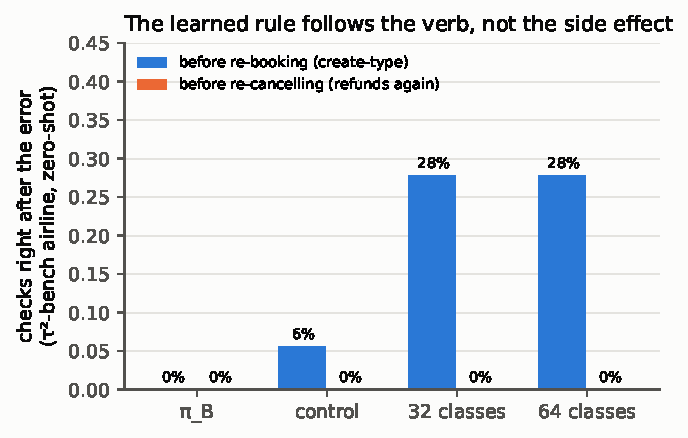
\includegraphics[width=0.48\linewidth]{figures/fig3_tau2_by_function.pdf}
\caption{Left: held-out-class success under the implicit timeout (bars = mean, dots = seeds). Right: zero-shot on \tautwo{} airline, checks before re-booking vs re-cancelling.}\label{fig:scale}
\end{figure}

\paragraph{But the learned rule follows verbs, not side effects.} Zero-shot on \tautwo{} airline, the synthetic-trained models check before re-booking (10/36) but never before re-cancelling (0/198). In every synthetic API, cancel-type calls were repeat-safe; \tautwo{}'s cancellation refunds again on every call, and its documentation does not say so. \textbf{Check-all-writes removes the shortcut.} Training the verb-agnostic rule ``after an uncertain failure of \emph{any} state-changing call, check, then decide'' (2 seeds) raises zero-shot \tautwo{} checking after the implicit timeout to 0.654 vs 0.026 ($+0.628$ [0.397, 0.859]), including 28/44 cancellations, and lifts BFCL held-out-class success to 0.829 ($+0.163$ [0.081, 0.236] over SYN-64) with no seed collapse. It does, however, regress the original suites (test 0.76--0.84 vs 0.87), concentrated in persistent-outage and impossible-request episodes: the training data never shows what to do when the re-issued call fails again, and the agent loops between checking and retrying. Under our pre-registered rule CAW was therefore not claimed. Adding 88 execution-verified \emph{persistent-failure continuations} (after a re-issued call fails again: switch to the backup endpoint, or escalate when the check itself keeps failing), at unchanged data size, gives \textbf{CAW-v2}, which meets every pre-registered condition (2 seeds): \tautwo{} zero-shot checking 0.846 vs 0.026 ($+0.821$ [0.667, 0.962]; 38/44 cancellations), BFCL held-out-class success 0.750 vs 0.667 ($+0.083$ [0.002, 0.155]), S1$|$S0 $\geq 0.95$, and the original suites within 0.01 of B (test 0.878 vs 0.872, held-out 0.727 vs 0.732; impossible-request success 1.00 vs 0.93). Relative to CAW it trades $-0.08$ on BFCL held-out for $+0.19$ on \tautwo{} and the removal of the regression.

\paragraph{Supervision form.} DPO variants regress ordinary behaviour (original test 0.74--0.80 vs 0.87 for B), whereas SFT stays within 0.02 of B on the original suites.

\section{Methodology}\label{sec:method}
\begin{itemize}
\item \textbf{Pre-registration.} Each study fixed its primary metric, matched baseline, single-seed futility gate and multi-seed claim rule before training. Changes made before results are appended to edit logs. Gates were applied as written, and four of six method studies were stopped at their gate.
\item \textbf{Execution verification} of every instance and training decision caught design errors before they reached results. One example: ``checks'' that cannot reveal the outcome without the earlier state, such as an account balance.
\item \textbf{Replication.} A single-seed pilot that favoured SFT over verified DPO reversed under three seeds.
\end{itemize}

\section{Limitations}
\begin{itemize}
\item \textbf{Scale of the base environment.} BFCL offers 8 API classes; the held-out-class sets have 9--35 tasks after conditioning on fault-free success.
\item \textbf{The \tautwo{} subset} is small (13 events) and uses forced-prefix episodes without the official user simulator. Fault-free completion there is 0.15, so check rates rather than success rates are informative.
\item \textbf{Model coverage.} All trained results use one model family (Qwen3-4B), and frontier API models are not evaluated.
\item \textbf{Fault placement.} Faults are injected at the first state-changing call only.
\end{itemize}

\section{Related work}
\begin{itemize}
\item \textbf{Tool-use benchmarks.} These measure call selection and parameterisation \citep{TODO_bfcl,TODO_apibank,TODO_toolllm} and stateful task completion \citep{TODO_taubench,TODO_tau2,TODO_appworld,TODO_toolsandbox}. Their faults, where present, have unambiguous correct responses.
\item \textbf{Corrective training.} Step-level corrective training for agents \citep{TODO_cso,TODO_skillcdpo} targets such faults. We reproduce a CSO-style baseline and show that it leaves uncertain outcomes untouched.
\item \textbf{Systems practice.} Idempotency and exactly-once semantics are standard in distributed systems \citep{TODO_idempotency}.
\item \textbf{Tool metadata and synthetic environments.} MCP tool annotations \citep{TODO_mcp} and procedurally generated tool environments \citep{TODO_synthetic} are related to our annotation and synthetic-API studies.
\item \textbf{Documentation.} We follow the Datasheets for Datasets template \citep{TODO_datasheets}.
\end{itemize}

\bibliographystyle{plainnat}
\bibliography{references}
\end{document}
